\let\negmedspace\undefined
\let\negthickspace\undefined
\documentclass[journal,12pt,onecolumn]{IEEEtran}
\usepackage[margin=2.5cm]{geometry} 
\usepackage{cite}
\usepackage{amsmath,amssymb,amsfonts,amsthm}
\usepackage{algorithmic}
\usepackage{graphicx}
\graphicspath{{./figs/}}
\usepackage{textcomp}
\usepackage{xcolor}
\usepackage{txfonts}
\usepackage{listings}
\usepackage{enumitem}
\usepackage{mathtools}
\usepackage{gensymb}
\usepackage{comment}
\usepackage{caption}
\usepackage[breaklinks=true]{hyperref}
\usepackage{tkz-euclide} 
\usepackage{listings}
\usepackage{gvv}  
\usepackage{gensymb}
\usepackage{multicol}
%\def\inputGnumericTable{}                                    
\usepackage{xparse}
\usepackage{color}                                            
\usepackage{array}                                            
\usepackage{longtable}                                       
\usepackage{calc}                                             
\usepackage{multirow}
\usepackage{multicol}
\usepackage{hhline}                                           
\usepackage{ifthen}                                           
\usepackage{lscape}
\usepackage{tabularx}
\usepackage{array}
\usepackage{float}
\newtheorem{theorem}{Theorem}[section]
\newtheorem{problem}{Problem}
\newtheorem{proposition}{Proposition}[section]
\newtheorem{lemma}{Lemma}[section]
\newtheorem{corollary}[theorem]{Corollary}
\newtheorem{example}{Example}[section]
\newtheorem{definition}[problem]{Definition}
\newcommand{\BEQA}{\begin{eqnarray}}
\newcommand{\EEQA}{\end{eqnarray}}
\newcommand{\define}{\stackrel{\triangle}{=}}
\theoremstyle{remark}
\newtheorem{rem}{Remark}

\begin{document}

\title{
GATE 2007\\
CH: CHEMICAL ENGINEERING}
\author{AI25BTECH11023 - Pratik R}
\maketitle
\renewcommand{\thefigure}{\theenumi}

\begin{enumerate}
   
    \item Given $i=\sqrt{-1}$, the ratio
\begin{align*}
    \frac{i+3}{i+1}
\end{align*}
is given by

\begin{enumerate}
    \item $i$
    \item $-2$
    \item $-i+2$
    \item $i+1$
\end{enumerate}

    \item The value of "a" for which the following set of equations
\begin{align*}
        y+2z &=0 \\
        2x+y+z &=0 \\
        ax+2y &=0
\end{align*}
has non trivial solution, is

\begin{enumerate}
    \item 0
    \item 8
    \item -2
    \item 3
\end{enumerate}

    \item The initial condition for which the following equation
    \begin{align*}
        \brak{x^2+2x}\frac{dy}{dx}=2\brak{x+1}y;\text{  }y\brak{x_0}=y_0
    \end{align*}
    has infinitely many solutions, is

\begin{enumerate}
    \item $y\brak{x=0}=5$
    \item $y\brak{x=0}=1$
    \item $y\brak{x=2}=1$
    \item $y\brak{x=-2}=0$
\end{enumerate}
\newpage
    \item Given that the Laplace transform of the function below over a single period $0<t<2$ is $\frac{1}{s^2}\brak{1-e^{-s}}^2$, the Laplace transform of the periodic function over $0<t<\infty$ is 
\begin{figure}[H]
    \centering
    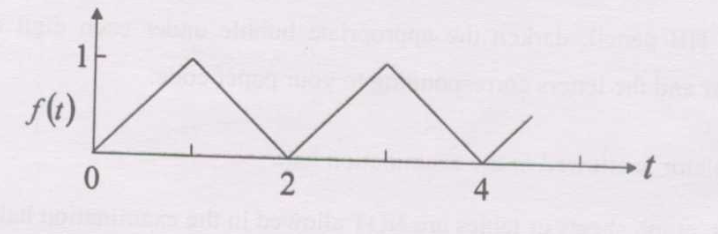
\includegraphics[width=0.5\columnwidth]{figs/4.png}
    \caption{}
    \label{fig:4}
\end{figure}

\begin{enumerate}
    \item $\frac{1}{s}\brak{1-e^{-s}}^2$
    \item $\frac{1}{s}\brak{1-e^{-s}}^2$
    \item $\frac{1}{s^2}\frac{1-e^{-s}}{1+e^{-s}}$
    \item $\frac{1}{s}tanh\frac{s}{2}$
\end{enumerate}

    \item If TA and TB are the boiling points of pure A and pure B respectively and $T_{AB}$ is that of a non homogeneous immiscible mixture of A and B, then

\begin{enumerate}
    \item $T_{AB}<T_A and T_B$
    \item $T_{AB}>T_A and T_B$
    \item $T_A>T_{AB}>T_B$
    \item $T_B>T_{AB}>T_A$
\end{enumerate}

    \item The state of an ideal gas is changed from (T1, P1) to (T2, P2) in a constant volume process. To calculate the change in enthalpy, $\Delta h$, ALL of the following properties/variables are required.

\begin{enumerate}
    \item $C_V,P_1,P_2$
    \item $C_P,T_1,T_2$
    \item $C_P,T_1,T_2,P_1,P_2$
    \item $C_V,P_1,P_2,T_1,T_2$
\end{enumerate}

    \item The change in entropy of the system, $\Delta S_{sys}$, undergoing a cyclic irreversible process is

\begin{enumerate}
    \item greater than 0
    \item equal to zero
    \item less than zero
    \item equal to the $\Delta S_{surroundings}$
\end{enumerate}

    \item Parameters 'a' and 'b' in the van der Waals and other cubic equations of state represent

\begin{enumerate}
    \item a -- molecular weight     b-- molecular polarity
    \item a -- molecular size       b -- molecular attraction
    \item a -- molecular size       b -- molecular speed
    \item a -- molecular attraction     b -- molecular size
\end{enumerate}

    \item  if $m_i, \Bar{m_i},m_i^R, m_i^E$ are molar, residual and excess properties respectively for a pure species "i", the mixture property M of a binary non ideal mixture of components 1 and 2, is given by
\begin{multicols}{2}
    \begin{enumerate}
        \item $x_1\Bar{m_1} + x_2\Bar{m_2}$     
        \item $x_1m_1^R + x_2m_2^R$
        \item $x_1m_1 + x_2m_2$
        \item $x_1m_1^E + x_2m_2^E$
    \end{enumerate}
\end{multicols}
\newpage
\item Consider a soap film bubble of diameter D. If the external pressure is $P_o$ and the surface tension of the soap film is $\sigma$, the expression for the pressure inside the bubble is

\begin{enumerate}
    \item $P_o$
    \item $P_o+\frac{2\sigma}{D}$
    \item $P_o + \frac{4\sigma}{D}$
    \item $P_o + \frac{8\sigma}{D}$
\end{enumerate}

    \item In Tyler series, the ratio of the aperture size of a screen to that of the next smaller screen is 

\begin{enumerate}
    \item $1/\sqrt{2}$
    \item $\sqrt{2}$
    \item $1.5$
    \item $2$
\end{enumerate}

    \item Size reduction of coarse hard solids using a crusher is accomplished by

\begin{enumerate}
        \item attrition
        \item compression
        \item cutting
        \item impact
\end{enumerate}

    \item In constant pressure filtration, the rate of filtration follows the relation (v: filtrate volume, t:time, k and c:constants).

\begin{enumerate}
    \item $\frac{dv}{dt}=kv+c$
    \item $\frac{dv}{dt}=\frac{1}{kv+c}$
    \item $\frac{dv}{dt}=kv$
    \item $\frac{dv}{dt}=kv^2$
\end{enumerate}

    \item Sticky materials are transported by

\begin{enumerate}
    \item apron conveyor
    \item screw conveyor
    \item belt conveyor
    \item hydraulic conveyor
\end{enumerate}

    \item The Grashof Number is

\begin{enumerate}
    \item thermal diffusivity/mass diffusivity
    \item inertial force/surface tension force
    \item sensible heat/latent heat
    \item buoyancy force/viscous force
\end{enumerate}

    \item An operator was told to control the temperature of a reactor at $60\degree C$. The operator set the set point of the temperature controller at 60. The scale actually indicated 0 to 100\% of a temperature range of 0 to $200\degree C$. This caused a runaway reaction by over pressurizing the vessel, which resulted in injury to the operator. The actual set point temperature was

\begin{enumerate}
    \item $200\degree C$
    \item $60\degree C$
    \item $120\degree C$
    \item $100\degree C$
\end{enumerate}
\newpage
    \item Select the most appropriate pump from Group2 to handle each fluid flow given in Group 1.

    \begin{multicols}{2}
        \begin{enumerate}[label =\Alph*]
            \item Highly viscous fluid flow
            \item Fluid containing large amount of abraisive solids
        \end{enumerate}
    \columnbreak
    \begin{enumerate}[label=\Roman*]
        \item piston pump
        \item gear pump
        \item plunger pump
        \item centrifugal pump
    \end{enumerate}
    \end{multicols}

\begin{enumerate}
    \item A-II, B-I
    \item A-II, B-IV
    \item A-III, B-IV
    \item A-IV, B-III
\end{enumerate}

    \item A cylinderical storage tank can have a self supported conical roof,

\begin{enumerate}
    \item if its diameter is less than 20m
    \item if its diameter is more than 20m
    \item if the thickness of the roof is more than that of the cylindrical shell 
    \item whatever is the diameter
\end{enumerate}

    \item Which of the following is desirable in gasoline but undesirable in kerosene?

\begin{enumerate}
    \item Aromatics
    \item Mercaptans
    \item Naphthenic Acid
    \item paraffins
\end{enumerate}

    \item In the Sulfite process for paper manufacture, the 'cooking liquor' is

\begin{enumerate}
    \item magnesium bisulfite and sulfur dioxide in acid medium
    \item magnesium sulfite and magnesium dicarbonate
    \item sodium sulfite and magnesium sulfite
    \item sodium sulfite, sodium bisulfite and sulfur dioxide
\end{enumerate}

    \item If $z=x+iy$ is a complex number, where $i=\sqrt{-1}$ then the derivative of $z\Bar{z}$ at $2+i$ is
\begin{multicols}{4}
\begin{enumerate}
    \item 0
    \item 2
    \item 4
    \item does not exist
\end{enumerate}
\end{multicols}
    \item $A$ and $B$ are two $3\times3$ matrix such  that 
    \begin{align*}
      A=  \myvec{
        -2 & 4 & 6 \\
        1 & 2 & 1 \\
        0 & 4 & 4 \\
        }, B = 0
    \end{align*}
and $AB=0$. then the rank of matrix $B$ is

\begin{multicols}{4}
    \begin{enumerate}
        \item $r=2$
        \item $r<3$
        \item $r \leq 3$
        \item $r=3$
    \end{enumerate}
\end{multicols}
\newpage
    \item The solution of the following differential equation 
    \begin{align*}
        x\frac{dy}{dx} + y\brak{x^2-1}= 2x^3
    \end{align*}
    is

\begin{multicols}{4}
    \begin{enumerate}
        \item $0$
        \item $2+ce^{-\frac{x^2}{2}}$
        \item $c_1x + c_2x^2$
        \item $2x+cxe^{-\frac{x^2}{2}}$
    \end{enumerate}
\end{multicols}

    \item The directional derivative of 
    \begin{align*}
        f=\frac{1}{2}\sqrt{x^2+y^2}
    \end{align*}
    at (1,1) in the direction of $\vec{b}=\hat{i} - \hat{j} $ is 

    \begin{multicols}{4}
    \begin{enumerate}
        \item 0
        \item $1/\sqrt{2}$
        \item $\sqrt{2}$
        \item $2$
    \end{enumerate}
    \end{multicols}

    \item Evaluate the following integral ($n\neq 0$)
    \begin{align*}
        \int_{c}\brak{-xy^n\,dx+x^ny\,dy}
    \end{align*}

within the area of a triangle with vertices (0,0),(1,0) and (1,1)(counter- clockwise)

\begin{multicols}{4}
    \begin{enumerate}
        \item 0
        \item $1/\brak{n+1}$
        \item $1/2$
        \item $n/2$
    \end{enumerate}
\end{multicols}

    \item The family of curves that is orthogonal to 
    \begin{align*}
        xy=c
    \end{align*}
    is
\begin{multicols}{4}
    \begin{enumerate}
        \item $y=c_1x$
        \item $y=c_1/x$
        \item $y^2+x^2=c_1$
        \item $y^2-x^2=c_1$
    \end{enumerate}
\end{multicols}

    \item The Laplace transform of
    \begin{align*}
        f(t)=1/\sqrt{t}
    \end{align*}
    is
    \begin{multicols}{4}
        \begin{enumerate}
            \item $\sqrt{\frac{\pi}{s}}$
            \item $\frac{1}{\sqrt{s}}$
            \item $\frac{1}{s^{\frac{3}{2}}}$
            \item does not exist
        \end{enumerate}
    \end{multicols}
    
    \item The thickness of a conductive coating in micrometers has a probability density function of $600x^{-2}$ for $100\mu m<x<120\mu m$. The meaning and the variance of the coating thickness is

    \begin{multicols}{2}
        \begin{enumerate}
            \item $1\mu m,108.39\mu m^2$
            \item $33.83\mu m,1\mu m^2$
            \item $105\mu m,11\mu m^2$
            \item $109.39\mu m,33.83\mu m^2$
        \end{enumerate}
    \end{multicols}

    \item If the percent humidity of air ($30\degree C$, total pressure 100kPa) is 24\% and the saturation pressure of water vapor at that temperature is 4kPa, the percent relative humidity and the absolute humidity of air are

    \begin{multicols}{4}
        \begin{enumerate}
            \item 25.2, 0.0062
            \item 25, 0.0035
            \item 20.7, 0.0055
            \item 18.2, 0.0035
        \end{enumerate}
    \end{multicols}

    \item For the two paths as shown in the figure, one reversible and one irreversible, to change the state of the system from a to b,
    \begin{figure}[H]
        \centering
        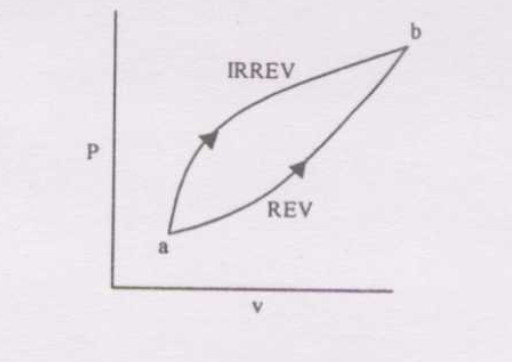
\includegraphics[width=0.5\columnwidth]{figs/30.png}
        \caption{}
        \label{fig:30}
    \end{figure}
\begin{multicols}{2}
    \begin{enumerate}
        \item $\Delta U,Q,W$ are same
        \item $\Delta U$ is same
        \item $Q, W$ are same
        \item $\Delta U, Q$ are different
    \end{enumerate}
\end{multicols}

    \item For a pure substance, the Maxewell's relation obtained from the fundamental property relation $du=Tds-Pdv$ is

\begin{multicols}{2}
    \begin{enumerate}
        \item $\brak{\partial T/\partial v}_s=-\brak{\partial P/\partial s}_v$
        \item $\brak{\partial P/\partial T}_v=\brak{\partial s/\partial v}_T$
        \item $\brak{\partial T/\partial P}_s=\brak{\partial v/\partial s}_P$
        \item $\brak{\partial v/\partial T}_P=-\brak{\partial s/\partial P}_T$
    \end{enumerate}
\end{multicols}

    \item Which of the following represents the Carnot cycle (ideal engine)?

\begin{multicols}{2}
    \begin{enumerate}
        \item \begin{figure}[H]
        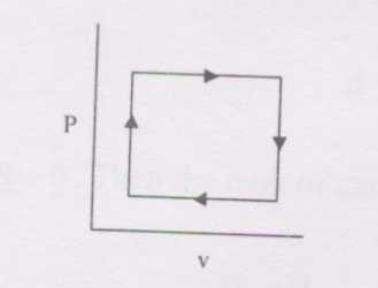
\includegraphics[width=0.4\linewidth]{figs/32a.png}
            \label{fig:32a}
        \end{figure}

        \item \begin{figure}[H]
        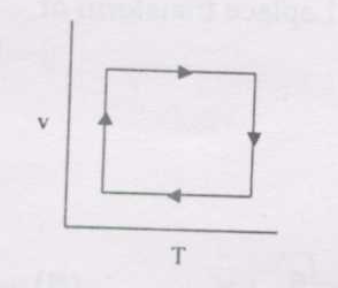
\includegraphics[width=0.4\linewidth]{figs/32b.png}
            \label{fig:32b}
        \end{figure}

        \item \begin{figure}[H]
        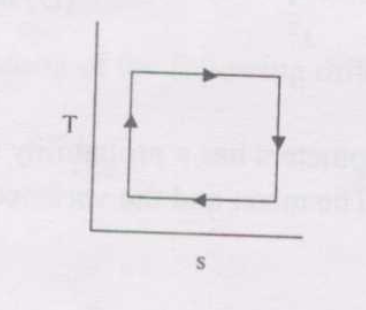
\includegraphics[width=0.4\linewidth]{figs/32c.png}
            \label{fig:32c}
        \end{figure}

        \item \begin{figure}[H]
        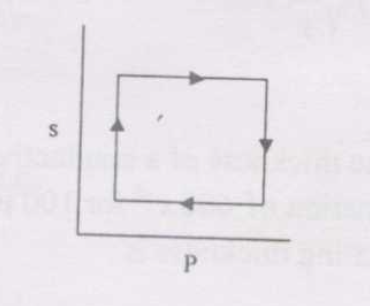
\includegraphics[width=0.4\linewidth]{figs/32d.png}
            \label{fig:32d}
        \end{figure}

    \end{enumerate}
\end{multicols}

    \item 2 kg of steam in a piston cylinder device at 400kPa and $175\degree C$ undergoes a mechanically reversible, isothermal compression to a final pressure such that the steam becomes just saturated. What is the work, W, required for the process.

    Data:

    $T=175\degree C$, $P = 400 kPa$ -- $v = 0.503 m^3/kg$, $u=2606kJ/kg$, $s=7.055 kJ/kgK$

    $T=175\degree C$, satd. vapor $= 400 kPa$ -- $v = 0.503 m^3/kg$, $u=2606kJ/kg$, $s=7.055 kJ/kgK$

\begin{multicols}{4}
    \begin{enumerate}
        \item 0 kJ
        \item 230 kJ
        \item 334 kJ
        \item 388 kJ
    \end{enumerate}
\end{multicols}

    \item Vapor phase hydration of  $C_2H_4$ to ethanol by the following reaction 
    \begin{align*}
    C_2H_4\brak{g}+H_2O\brak{g} \leftrightarrow C_2H_5OH\brak{g}
     \end{align*}
attains equilibrium at 400K and 3 bar. The standard Gibbs free energy change of reaction at these conditions is $\Delta g\degree = 4000J/mol$. For 2moles of an equimolar feed of ethylene and steam, the equation in terms of the extent of reaction $\epsilon$ (in mols) at equilibrium is 

\begin{multicols}{2}
    \begin{enumerate}
        \item $\frac{\epsilon \brak{2-\epsilon}}{\brak{1 - \epsilon}^2} - 0.3 =0$
        \item $\frac{\brak{1-\epsilon}^2}{\epsilon \brak{2 - \epsilon}} - 0.9 =0$
        \item $\frac{\epsilon}{\brak{1 - \epsilon}^2} - 0.3 =0$
        \item $\frac{\epsilon \brak{2-\epsilon}}{\brak{1 - \epsilon}^2} - 0.9 =0$
    \end{enumerate}
\end{multicols}

    \item A pipeline system carries crude oil of density $800kg/m^3$. The volumetric flow rate at point 1 is $0.28 m^3/s$. The cross sectional areas of the branches 1,2 and 3 are 0.012, 0.008 and 0.004 $m^2$ respectively. All the three branches are in a horizontal plane and the friction is negligible. If the pressure at the points 1 and 3 are 270 kPa and 240kPa respectively, then the pressure at point 2 is 

    \begin{figure}[H]
    \centering
        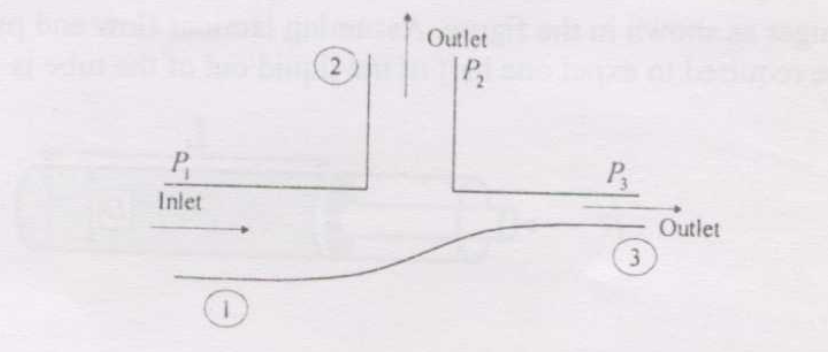
\includegraphics[width=0.5\columnwidth]{figs/35.png}
        \caption{}
        \label{fig:35}
    \end{figure}

\begin{multicols}{4}
    \begin{enumerate}
        \item 202 kPa
        \item 240 kPa 
        \item 284 kPa
        \item 355 kPa
    \end{enumerate}
\end{multicols}

    \item The figure shows the idealized view of a return elbow or U bend, which is connected to two pipes by flexible hoses that transmit no force. Water with density $1000 kg/m^3$ flows at velocity of 10 m/s through the pipe, which has a uniform ID of 0.1m. The gauge pressure at points 1 and 2 are 304 kPa and 253 kPa respectively. The horizontal force $F$ required to keep the elbow in position is 

\begin{figure}[H]
    \centering
    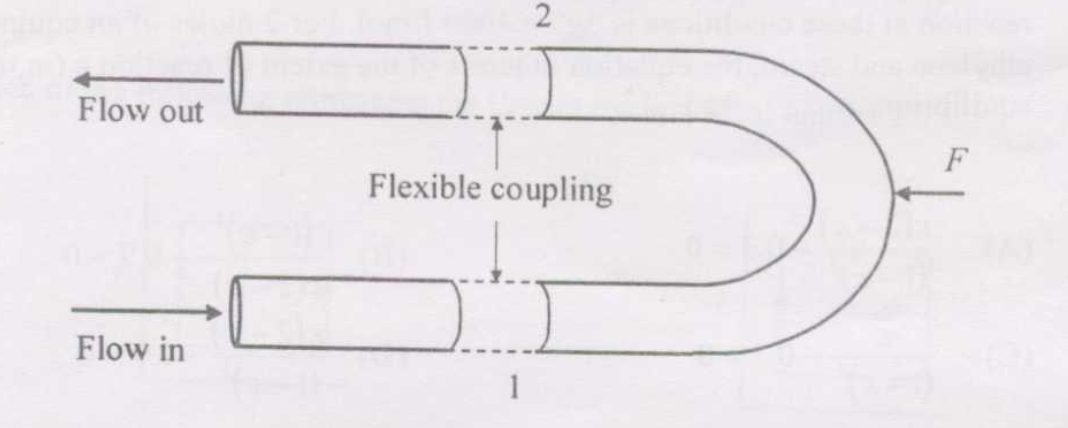
\includegraphics[width=0.5\columnwidth]{figs/36.png}
    \caption{}
    \label{fig:36}
\end{figure}

\begin{multicols}{4}
    \begin{enumerate}
        \item 1574 N
        \item 1970 N
        \item 5942 N
        \item 7533 N
    \end{enumerate}
\end{multicols}

    \item A tube of diameter D and length L is initially filled with a liquid of density $\rho$ and viscosity $\mu$. It is then pushed out by the application of a constant force $F$ to the plunger as shown in the figure. Assuming laminar flow and pseudo steady state, the time required to expel one half of the liquid out of the tube is 

    \begin{figure}[H]
        \centering
        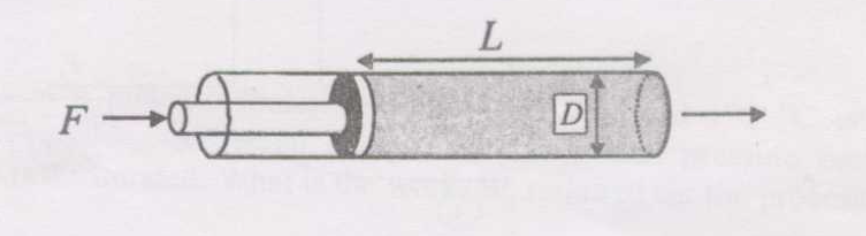
\includegraphics[width=0.5\columnwidth]{figs/37.png}
        \caption{}
        \label{fig:37}
    \end{figure}

    \begin{enumerate}
        \item $\frac{3\pi \mu L^2}{F}$
        \item $\frac{3\pi \mu D^2}{F}$
        \item $\frac{3\pi \mu L^2}{F}$
        \item $\frac{6\pi \mu D L}{F}$
    \end{enumerate}

    \item The figure shows a series parallel configuration of three identical centrifugal pumps. The head increase $\Delta H$ across a single such pump varies with flowrate $Q$ according to $\Delta H=a-bQ^2$. The expression for the total head increase $\Delta H=H_2 - H_1$ in terms of $a$ and $b$ and the total flowrate $Q_1$ for this configuration is given by 

    \begin{figure}[H]
        \centering
        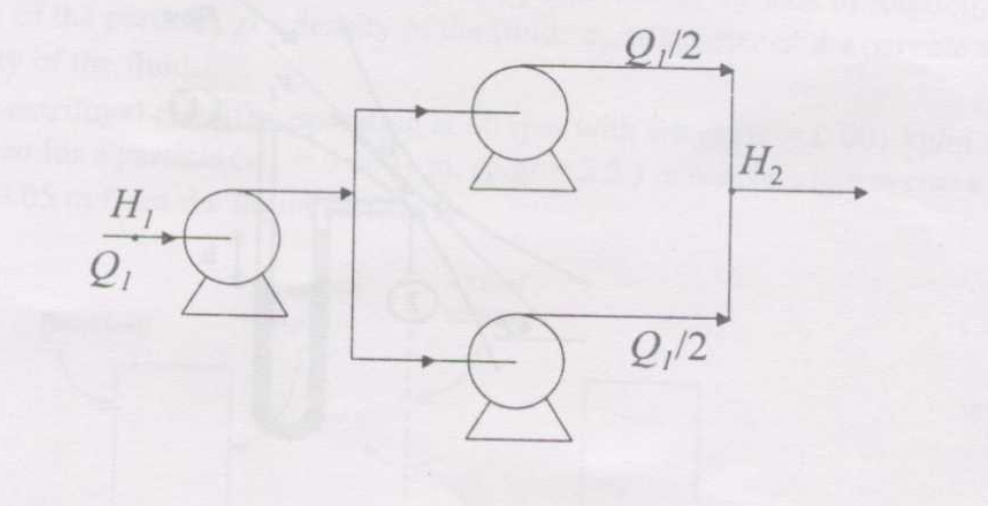
\includegraphics[width=0.5\columnwidth]{figs/38.png}
        \caption{}
        \label{fig:38}
    \end{figure}

\begin{enumerate}
    \item $2a-\frac{5}{4}bQ^2_1$
    \item $2a-bQ_1^2$
    \item $2a-2bQ_1^2$
    \item $a-bQ_1^2$
\end{enumerate}

    \item The pressure differential across a venturimeter, inclined at $45\degree $ to the vertical (as shown in the figure) is measured with the help of a manometer to estimate the flowrate of a fluid flowing through it. If the density of the flowing fluid is $\rho$ and the density of the manometer fluid is $\rho_m$, the velocity of the fluid at the throat can be obtained from expression

\begin{figure}[H]
    \centering
    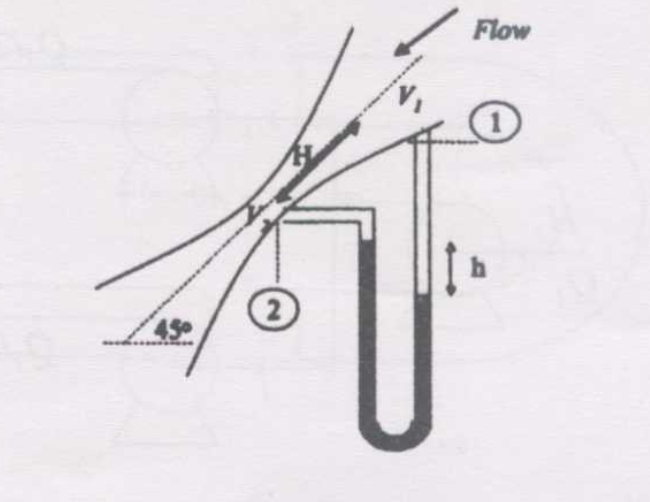
\includegraphics[width=0.5\linewidth]{figs/39.png}
    \caption{}
    \label{fig:39}
\end{figure}

\begin{enumerate}
    \item $\frac{V_2^2-V_1^2}{2g}=\frac{h\brak{\rho _m-\rho}}{\rho}+Hsin45\degree $
     \item $\frac{V_2^2-V_1^2}{2g}=\frac{h\rho_m}{\rho}+Hsin45\degree $
      \item $\frac{V_2^2-V_1^2}{2g}=\frac{h\rho _m}{\rho}$
      \item $\frac{V_2^2-V_1^2}{2g}=\frac{h\brak{\rho_m-\rho}}{\rho}$
\end{enumerate}
\newpage
    \item In the Stokes regime, the velocity of particles for centrifugal sedimentation is given by 
    \begin{align*}
        U_t=\omega^2r\brak{\rho_p-\rho}d^2_p/18\mu
    \end{align*}
    where, $\omega$ :angular velocity; $r$ : distance of the particle from the axis of rotation; $\rho_p$ : density of the particle; $\rho$  : density of the fluid; $d_p$ : diameter of the particle and $\mu$ : viscosity of the fluid.

    In a Bowl centrifugal classifier operating at 60 rpm with water $\brak{\mu = 0.001 kg/m.s}$, the time taken for a particle $\brak{d_p = 0.0001 m, sp.gr=2.5}$ in seconds to traverse a distance of 0.05 m from the liquid surface is

    \begin{figure}[H]
        \centering
        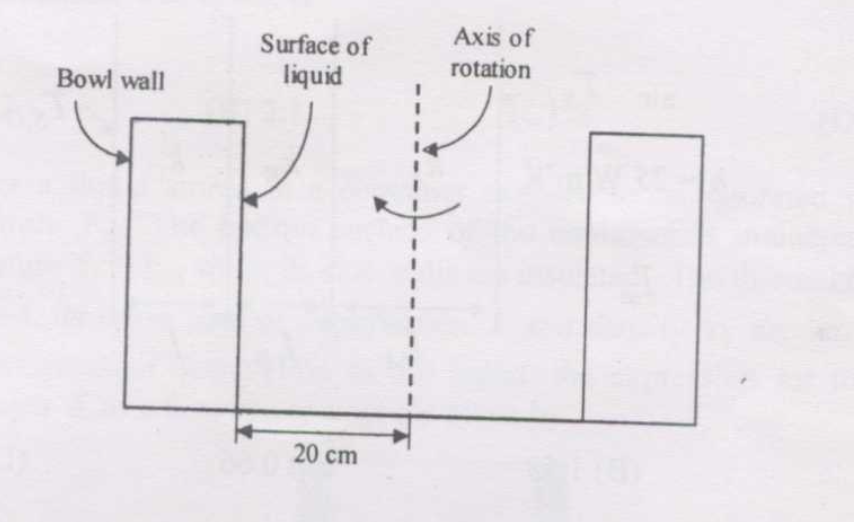
\includegraphics[width=0.5\columnwidth]{figs/40.png}
        \caption{} 
        \label{fig:40}
    \end{figure}

\begin{multicols}{4}
    \begin{enumerate}
        \item 4.8
        \item 5.8
        \item 6.8
        \item 7.8
    \end{enumerate}
\end{multicols}

    \item For the two long concentric cylinders with surface areas $A_1$ and $A_2$, the view factor $F_{22}$ is given by

    \begin{figure}[H]
        \centering
        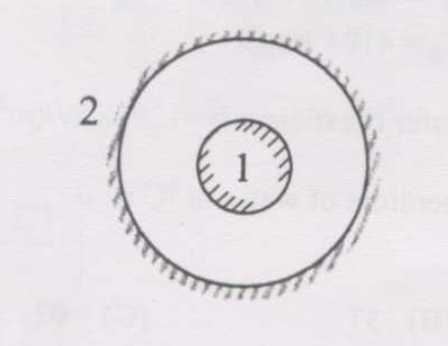
\includegraphics[width=0.5\columnwidth]{figs/41.png}
        \caption{}
        \label{fig:41}
    \end{figure}

\begin{multicols}{4}
    \begin{enumerate}
        \item 0
        \item 1
        \item 1 - $A_1/A_2$
        \item $A_1/A_2$
    \end{enumerate}
\end{multicols}

    \item The composite wall of an oven consists of three materials A, B and C. Under steady state operating conditiond, the outer surface temperature $T_{so}$ is $20\degree C$, the inner surface temperature $T_{si}$ is $600\degree C$ and the oven air temperature is $T_\infty = 800\degree C$. For the following data 

    thermal conductivities $k_A=20 W/\brak{mK}$ and $k_C=50W/\brak{mK}$,

    thickness $L_A=0.3m$, $L_B=0.15m$ and $L_C=0.15m$,
    inner wall heat transfer coeeficient $h=25W/\brak{m^2K}$

    the thermal conductivity $k_B$ (W/(mK) of the material B, is calculated as 

    \begin{figure}[H]
        \centering
        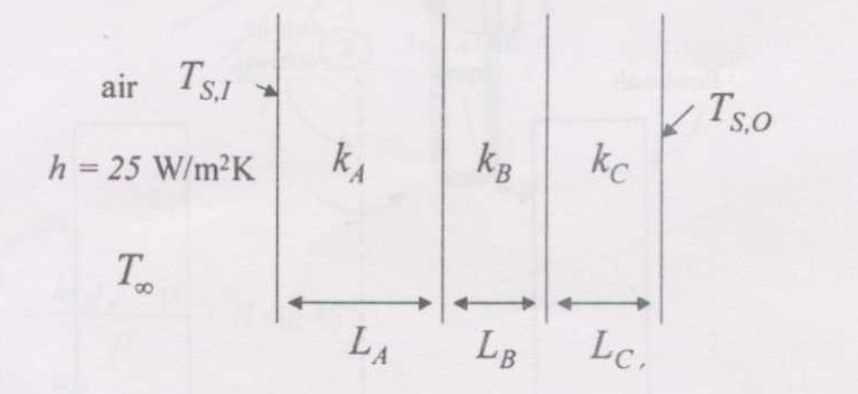
\includegraphics[width=0.5\columnwidth]{figs/42.png}
        \caption{}
        \label{fig:42}
    \end{figure}

\begin{multicols}{4}
    \begin{enumerate}
        \item 35
        \item 1.53
        \item 0.66
        \item 0.03
    \end{enumerate}
\end{multicols}
    
    \item Water enters a thin walled tube(L=1 m, D=3 mm) at an inlet temperature of $27\degree C$. Given the following data for water

    \begin{align*}
        \text{Density}, \rho &= 1000 kg/m^3 \\
        \text{Viscosity}, \mu &= 489\times 10^{-6} Ns/m^2 \\
        \text{Specific heat}, C_p &= 4184 J/kg/k \\
    \end{align*}
    Inside heat transfer coefficient h = 12978 W/($m^2K$),
    
    the outlet temperature of water in $\degree C$ is.
\begin{multicols}{4}
    \begin{enumerate}
        \item 28
        \item 37
        \item 62
        \item 96
    \end{enumerate}
\end{multicols}

    \item A hot fluid entering a well stirred vessel is cooled by feeding cold water through a jacket around the vessel. Assume the jacket is well mixed. For the following data,

    \begin{enumerate}[label =]
        \item mass flowrates of the hot fluid = 0.25 kg/s,
        \item mass flow rate of cold water = 0.4 kg/s
        \item specific heats of oil = 6000 J/kgK
        \item specific heat of cold water = 4184 J/kgK
        \item the inlet and exit temperature of the hot fluid is $150\degree C$ and $100\degree C$ respectively.
        \item inlet temperature of cold water = $20\degree C$
        \item the overall heat transfer coefficient is $500 W/m^2K$
    \end{enumerate}
the heat transfer area in $m^2$, is 
\begin{multicols}{4}
    \begin{enumerate}
        \item 1.82
        \item 2.1
        \item 3
        \item 4.26
    \end{enumerate}
\end{multicols}

    \item Consider a liquid stored in a container exposed to its saturated vapor at constant temperature $T_{sat}$. The bottom surface of the container is maintained at a constant temperature $T_s<T_{sat}$ while its side walls are insulated. The thermal conductivity $k_1$ of the liquid, its latent heat of vaporisation $\lambda$ and density $\rho_1$ are known. Assuming a linear temperature distribution in the liquid, the expression for the growth of the liquid layer $\delta$ as a function of time $t$ is given by

    \begin{figure}[H]
        \centering
        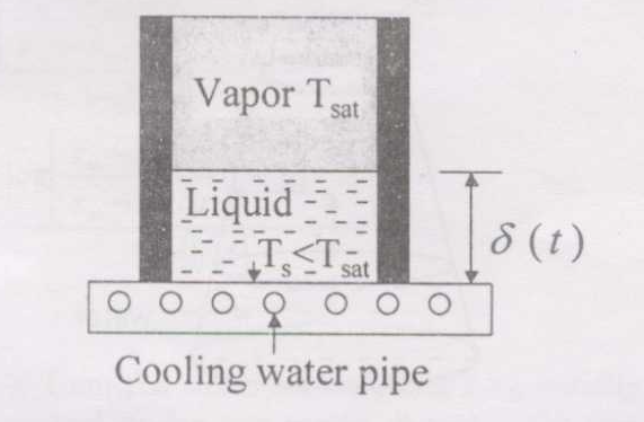
\includegraphics[width=0.5\columnwidth]{figs/45.png}
        \caption{}
        \label{fig:45}
    \end{figure}
\begin{enumerate}
    \item $\delta \brak{t}=\sbrak{\frac{4k_1\brak{T_{sat}-T_{s}}}{\rho_1 \lambda}t}^{1/2}$
    \item $\delta \brak{t}=\sbrak{\frac{k_1\brak{T_{sat}-T_{s}}}{2\rho_1 \lambda}t}^{1/2}$
    \item $\delta \brak{t}=\sbrak{\frac{2k_1\brak{T_{sat}-T_{s}}}{\rho_1 \lambda}t}^{1/2}$
    \item $\delta \brak{t}=\sbrak{\frac{k_1\brak{T_{sat}-T_{s}}}{\rho_1 \lambda}t}^{1/2}$
\end{enumerate}
   
   \item The following list of options P,Q,R and S are some of the important considerations in the design of a shell and tube heat exchsnger.

   \begin{enumerate}
       \item[P] square pitch permits the use of more tubes in a given shell diameter
       \item[Q] the tube side clearance should not be less than one fourth of the tube diameter
       \item[R] baffle spacing is not greater than the diameter of the shell or less than one fifth of the shell diamter
       \item[S] The pressure drop on the tube side is less than 10psi
   \end{enumerate}
   
    \item Pick out the correct combination of 'TRUE' statements from the following:

    \begin{enumerate}
        \item P, Q and R
        \item Q, R and S
        \item R, S and P
        \item P, Q, R and S
    \end{enumerate}
   
   \item The following figure depicts steady one-dimensional diffusion of water vapour from the surface of water taken in a conical flask at room temperature. Derive the governing equation for determining the concentration profile of water vapour in the gas medium. Neglect change of level of water due to condensation. The temperatures of the gas and the liquid media are identical and constant.

   \begin{figure}[H]
       \centering
       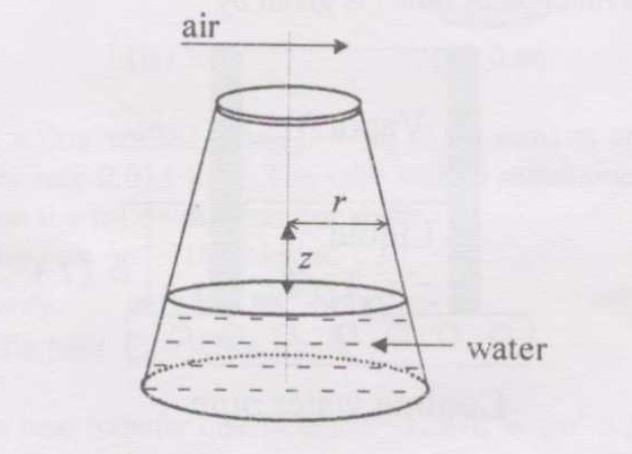
\includegraphics[width=0.5\columnwidth]{figs/47.png}
       \caption{}
       \label{fig:47}
   \end{figure}

\begin{enumerate}
    \item $\frac{d}{dz}\sbrak{r^2\frac{CD_{WA}}{1-x_W}\frac{dx_W}{dz}}=0$
    \item $\frac{d}{dz}\sbrak{\frac{CD_{WA}}{1-x_W}\frac{dx_W}{dz}}=0$
    \item $\frac{d}{dz}\sbrak{r\frac{CD_{WA}}{1-x_W}\frac{dx_W}{dz}}=0$
    \item $\frac{d}{dz}\sbrak{rCD_{WA}\frac{dx_W}{dz}}=0$
\end{enumerate}

   \item In a distillation operation, it is desired to have a very high purity bottom product. Initially, a kettle-type reboiler is used at the bottom of the column and the following analytical equation is used to obtain the equilibrium trays in the exhausting section of the column
   \begin{align*}
       N_P-m+1=\frac{\log\sbrak{\frac{x_m-x_w/\alpha}{x_w-x_w/\alpha}\brak{1-\Bar{A}}+\Bar{A}}}{\log \brak{1/\Bar{A}}}
   \end{align*}
   
   where x is the composition of the liquid leaving tray m. Tray m is the last equilibrium tray obtained by a McCabe Thiele graph of the exhausting section. If the kettle type reboiler is replaced by a thermo syphon reboiler, the analytical equation, for the exhausting section will be

\begin{enumerate}
    \item $  N_P-m+1=\frac{\log\sbrak{\frac{x_m-x_w/\alpha}{x_w-x_w/\alpha}\brak{1-\Bar{A}}+\Bar{A}}}{\log \brak{1/\Bar{A}}}$
    \item $  N_P+1=\frac{\log\sbrak{\frac{x_m-x_w/\alpha}{x_w-x_w/\alpha}\brak{1-\Bar{A}}+\Bar{A}}}{\log \brak{1/\Bar{A}}}$
     \item $  N_P-m=\frac{\log\sbrak{\frac{x_m-x_w/\alpha}{x_w-x_w/\alpha}\brak{1-\Bar{A}}+\Bar{A}}}{\log \brak{1/\Bar{A}}}$
      \item $  N_P-m+2=\frac{\log\sbrak{\frac{x_m-x_w/\alpha}{x_w-x_w/\alpha}\brak{1-\Bar{A}}+\Bar{A}}}{\log \brak{1/\Bar{A}}}$
\end{enumerate}
   
    \item A $50cm \times 50 cm \times 1 cm$ flat wet sheet weighing 2 kg initially, was dried from both the sides under constant drying rate period. It took 1000 secs for the weight of the sheet to reduce to 1.75 kg. Another $1m\times 1m\times 1cm$ flat sheet is to be dried from one side only. Under the same drying rate and other conditions, time required for drying (in secs) from initial weight of 4 kg to 3 kg is 

    \begin{multicols}{4}
        \begin{enumerate}
    \item 1000
    \item 1500
    \item 2000
    \item 2500
\end{enumerate}
    \end{multicols}

    \item It is desired to reduce the concentration of pyridine in 500kg of aqueous solution from 20 weight percent to 5wt percent in a single batch extraction using chlorobenzene as solvent. Equilibrium compositions(end points of the tie line) in terms of weight percent of pyridine water chlorobenzene are (5,95,0) and (11,0,89).

    The amount of pure solvent required in kg for the operation is

    \begin{multicols}{4}
        \begin{enumerate}
            \item 607
            \item 639
            \item 931
            \item 1501
        \end{enumerate}
    \end{multicols}

    \item Benzene in air benzene mixture is to be reduced from $5.2mol\%$ in the feed to $0.5mol\%$
 by contacting with wash oil in a multistage countercurrent gas absorber. The inlet flowrate of air benzene mixture is 10mol/s while benzene free wash oil comes in at 9.5 mol/s. If the equilibrium curve is given as $Y^*$ and $X$ are equilibrium mole ratios of benzene in air and benzene in oil, the number of equilibrium stages required to achieve the above seperation is 

 \begin{figure}[H]
     \centering
     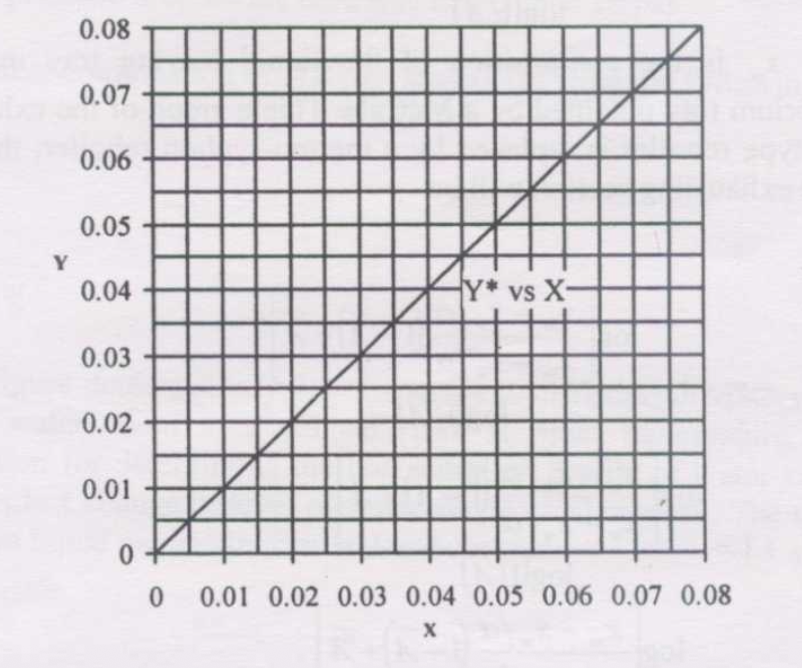
\includegraphics[width=0.5\columnwidth]{figs/51.png}
     \caption{}
     \label{fig:51}
 \end{figure}

 \begin{multicols}{4}
     \begin{enumerate}
         \item 12
         \item 10
         \item 8
         \item 6
     \end{enumerate}
 \end{multicols}
 
    \item A well stirred reaction vessel is operated as a semi batch reactor in which it is proposed to conduct a liquid phase first order reaction of the type $A\to B$. The reactor is fed with the reactant A at  a constant rate of 1 liter/min having feed concentration equal to 1mol/liter. The reactor is initially empty. Given $k=1min^{-1}$, the conversion of reactant A based on moles of A fed at $t=2min$ is

    \begin{multicols}{4}
        \begin{enumerate}
            \item 0.136
            \item 0.43
            \item 0.57
            \item 0.864
        \end{enumerate}
    \end{multicols}

 \item A liquid phase exothermic first order reaction is being conducted in a batch reactor under isothermal conditions by removing heat generated in the reactor with the help of cooling water. The cooling water flows at a very high rate through a coil immersed in the reactor such that there is negligible rise in its temperature from inlet to outlet of the coil. If the rate constant is given as $k$, heat of reaction(-$\Delta H$), volume of the reactor, $V$, initial concentration as $C_{}A0$, overall heat transfer coefficient, $U$, heat transfer area of the coil is equal to A, the required cooling water inlet temperature, $T_{ci}$ is given by the following equation:

 \begin{enumerate}
     \item $T_{ci}=T-\frac{\brak{-\Delta H}VkC_{A0}}{UA}$
      \item $T_{ci}=T-\frac{\brak{-\Delta H}VkC_{A0}e^{-kt}}{UA}$
       \item $T_{ci}=T-\frac{\brak{-\Delta H}VC_{A0}e^{-kt}}{UAt}$
        \item $T_{ci}=T-\frac{\brak{-\Delta H}VC_{A0}}{UAt}$
 \end{enumerate}

    \item The following liquid phase reaction is taking place in an isothermal CSTR
    \begin{align*}
        A\xrightarrow{k_1}B\xrightarrow{k_2}C \\
        2A\xrightarrow{k_3}D
    \end{align*}

Reaction mechanism is same as the stoichiometry given above. Given $k_1 min^{-1}$; $k_2=1min^{-1}$; $k_3=0.5 lit/mol\cdot min$; $C_{A0}=10mol/litre$, $C_{B0}=0mol/litre$ and $C_B=1mol/litre$, the solution for F/V(flow rate/reactor volume in $min^{-1}$) yields

\begin{multicols}{4}
    \begin{enumerate}
        \item 6.7
        \item 6 and 0.5
        \item 2 and 4/3
        \item 8
    \end{enumerate}
\end{multicols}
    
    \item A pulse of concentrated KCL solution is introduced as tracer into the fluid entering a reaction vessel having volume equal to $1m^{3}$ and flow rate equal to $1m^{3}/min$. The concentration of tracer measured in the fluid leaving the vessel is shown in the figure given below. The flow model parameters that fit the measured RTD in terms of one or all of the following mixing elements, namely, volume of plug flow reactor, $V_p$, mixed flow volume, $V_m$, and dead space, $V_d$, are
    \begin{figure}[H]
        \centering
        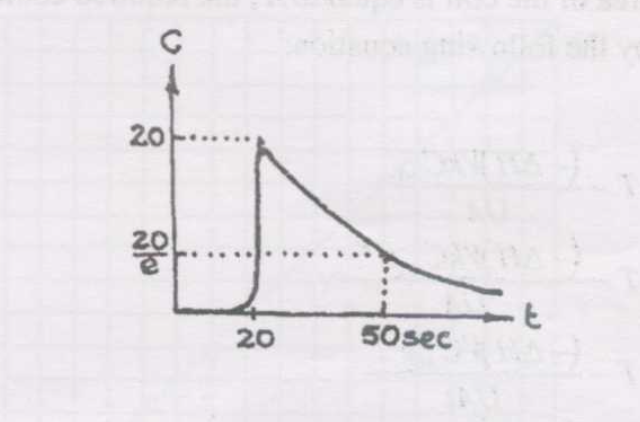
\includegraphics[width=0.5\columnwidth]{figs/55.png}
        \caption{}
        \label{fig:55}
    \end{figure}
 
    \item The first order reaction of A to R is run in an experimental mixed flow reactor. Find the role played by pure diffusion in the run given below. $C_A0$ is 100 and W is fixed. Agitation rate was found to have no effect on conversion.

    \begin{multicols}{3}
         \begin{enumerate}[label =]
             \item $d_p$
             \item 4
             \item 6
         \end{enumerate}
         \columnbreak
         \begin{enumerate}[label =]
             \item $F_{A0}$
             \item 2
             \item 4
         \end{enumerate}
         \columnbreak
         \begin{enumerate}[label =]
             \item $X_A$
             \item 0.8
             \item 0.4
         \end{enumerate}
    \end{multicols}

 \begin{enumerate}
     \item strong pure diffusion control
     \item diffusion free
     \item intermediate role by pure diffusion
     \item external mass transfer
 \end{enumerate}

    \item A packed bed reactor converts A to R by first order reaction with 9mm pellets in strong pure diffusion regime to 63.2\% level. If 18mm pellets are used what is the conversion.

    \begin{multicols}{4}
        \begin{enumerate}
            \item 0.39
            \item 0.61
            \item 0.632
            \item 0.865
        \end{enumerate}
    \end{multicols}

    \item The following rate concentration data are calculated from experiment. Find the activation energy temperature(E/R) of the first order reaction.

    \begin{multicols}{4}
        \begin{enumerate}[label =]
            \item $d_p$
            \item $1$
            \item $2$
            \item $2$
        \end{enumerate}
        \columnbreak
        \begin{enumerate}[label =]
            \item $C_A$
            \item $20$
            \item $40$
            \item $40$
        \end{enumerate}
        \columnbreak
        \begin{enumerate}[label =]
            \item $-r_A$
            \item 1
            \item 2
            \item 3
        \end{enumerate}
        \columnbreak
        \begin{enumerate}[label =]
            \item T
            \item 480
            \item 480
            \item 500
        \end{enumerate}
    \end{multicols}

\begin{multicols}{4}
    \begin{enumerate}
        \item 2432.8
        \item 4865.6
        \item 9731.2
        \item 13183.3
    \end{enumerate}
\end{multicols}

    \item Determine the level of $C_{A0}$(high, low, intermediate), temperature profile (high, low, increasing, decreasing) which will favor the formation of the desired product indicated in the reaction schemes given below.

    \begin{align*}
        A\xrightarrow{1}R\xrightarrow{3}S_{desired} \\
        A\xrightarrow{2}U
    \end{align*}

    \begin{multicols}{6}
        \begin{enumerate}[label =]
            \item $n_1$
            \item 2
        \end{enumerate}
        \columnbreak
        \begin{enumerate}[label =]
            \item $E_1$
            \item 25
        \end{enumerate}
        \columnbreak
    \begin{enumerate}[label =]
        \item $n_2$
        \item 1
    \end{enumerate}
    \columnbreak
    \begin{enumerate}[label =]
        \item $E_2$
        \item 35
    \end{enumerate}
    \columnbreak
    \begin{enumerate}[label =]
        \item $n_3$
        \item 3
    \end{enumerate}
    \columnbreak
    \begin{enumerate}[label =]
        \item $E_3$
        \item 45
    \end{enumerate}
    \end{multicols}

\begin{enumerate}
    \item High $C_{A0}$, increasing T, plug flow reactor
      \item High $C_{A0}$, increasing T, plug flow reactor
        \item High $C_{A0}$, increasing T, plug flow reactor
          \item High $C_{A0}$, increasing T, plug flow reactor
\end{enumerate}
\newpage
    \item The dynamic model for a mixing tank open to atmosphere at its top as shown below is to be written. The objective of mixing is to cool the hot water stream entering the tank at a flow rate $q_2$ and feed temperature of $T_s$ with a cold water feed stream entering the tank at a flow rate $q_1$ and feed temperature of $T_0$. A water stream is drawn from the tank bottom at a flow rate of $q_4$ by a pump and the level in the tank is proposed to be controlled by drawing another water stream at a flow rate $q_3$. Neglect evaporation and other heat losses from the tank
\begin{figure}[H]
    \centering
    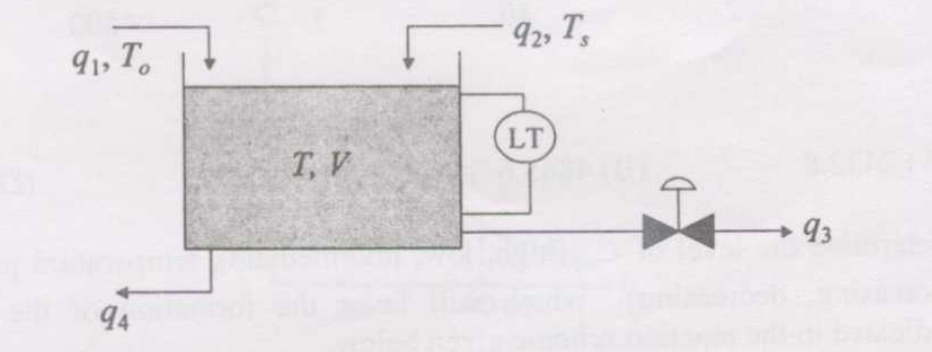
\includegraphics[width=0.5\columnwidth]{figs/60.png}
    \caption{}
    \label{fig:60}
\end{figure}

    The dynamic model for the tank is given as

\begin{enumerate}
    \item $\frac{dV}{dt} = q_1 + q_2 - q_3,$ \hspace{1cm} $V\frac{dT}{dt} = q_1T_o + q_2T_s - q_3T$
    \item $\frac{dV}{dt} = q_1 - q_4,$ \hspace{1cm} $\frac{d(VT)}{dt} = q_1T_s - q_4T$
    \item $\frac{dV}{dt} = q_1 + q_2 - q_4,$ \hspace{1cm} $\frac{d(VT)}{dt} = q_1T_o + q_2T_s - q_4T$
    \item $\frac{dV}{dt} = q_1 + q_2 - q_3 - q_4,$ \hspace{1cm} $V\frac{dT}{dt} = q_1(T_o - T) + q_2(T_s - T)$
\end{enumerate}
\newpage
    \item Match the transfer functions with the responses to a unit step input shown in the figure.
\begin{figure}[H]
    \centering
    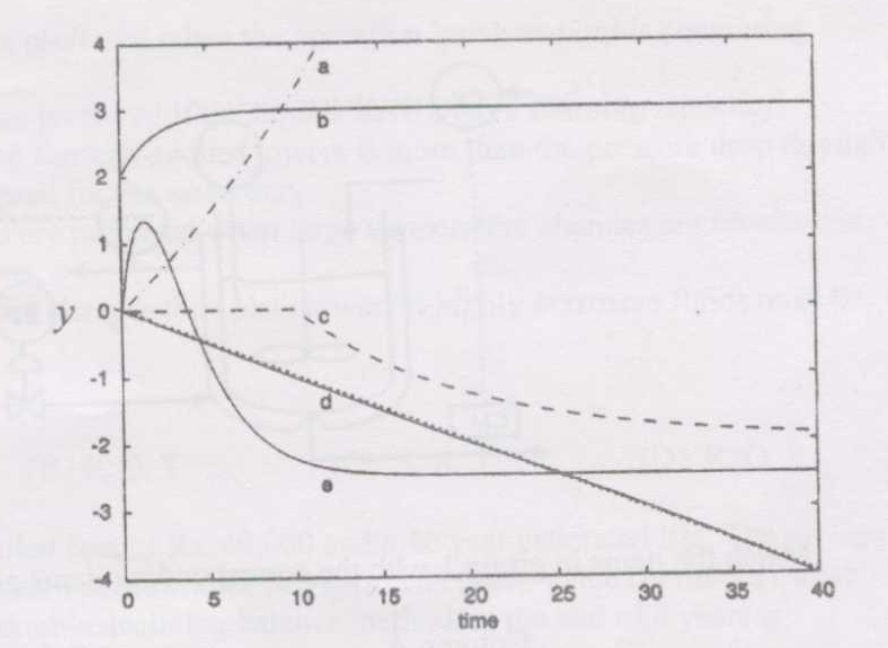
\includegraphics[width=0.5\columnwidth]{figs/61.png}
    \caption{}
    \label{fig:61}
\end{figure}
    \begin{enumerate}[label =\roman*]
    \item $ \dfrac{-2.5(-4s+1)}{4s^2 + 4s + 1} $
    \item $ \dfrac{-2e^{-10s}}{10s+1} $
    \item $ \dfrac{-5}{-20s+1} $
    \item $ \dfrac{-0.1}{s} $
    \item $ \dfrac{4s+3}{2s+1} $
\end{enumerate}

\begin{enumerate}
    \item i-e, ii-c, iii-a, iv-d, v-b
    \item i-a, ii-b, iii-c, iv-d, v-e
    \item i-b, ii-a, iii-c, iv-e, v-d
    \item i-e, ii-a, iii-c, iv-b, v-d
\end{enumerate}

    \item consider the following instrumentation diagram for a chemical reactor.  $C_{sp}$ represents a concentration setpoint.

    \begin{figure}[H]
        \centering
        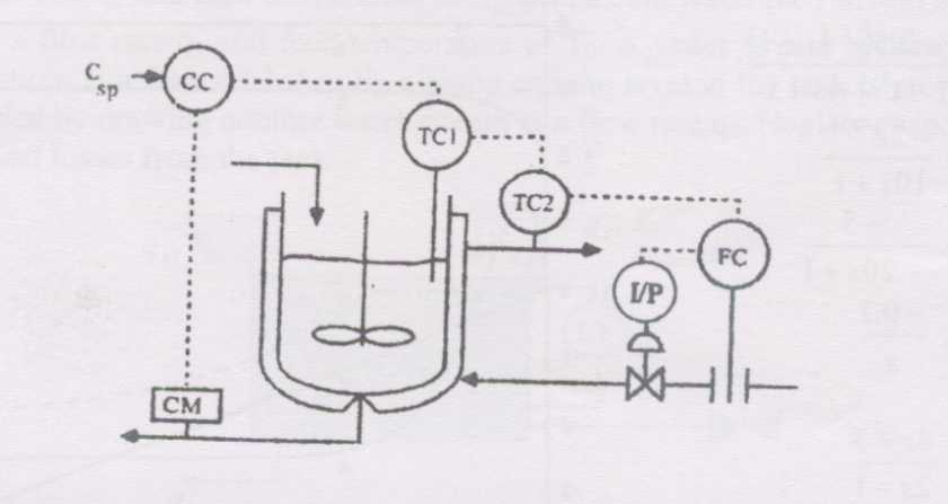
\includegraphics[width=0.5\columnwidth]{figs/62.png}
        \caption{}
        \label{fig:62}
    \end{figure}
Match the items in group 1 with the corresponding items given in column B.

\begin{multicols}{2}
\textbf{Column A}
\begin{enumerate}
    \item P) control strategy
    \item Q) primary control variable
    \item R) slowest controller
    \item S) fastest controller
\end{enumerate}

\columnbreak

\textbf{Column B}
\begin{enumerate}
    \item feed forward control
    \item cascade control
    \item concentration in the reactor
    \item reactor temperature
    \item jacket temperature
    \item concentration controller
    \item reactor temperature controller
    \item jacket temperature controller
    \item flow controller
    \item selective control
\end{enumerate}
\end{multicols}

\begin{multicols}{2}
\begin{enumerate}
    \item P-2, Q-3, R-6, S-9
    \item P-1, Q-4, R-8, S-7
    \item P-10, Q-7, R-9, S-6
    \item P-1, Q-8, R-5, S-9
\end{enumerate}
\end{multicols}
    \item 

The first two rows of Routh's tabulation of a third order equation are

\begin{table}[H]
\centering
\begin{tabularx}{0.5\textwidth}{|l|X|X|}
\hline
\textbf{} & \textbf{M1} & \textbf{M2} \\
\hline
Purchase cost(in lakhs of rupees) & 10 & 5 \\
\hline
Expected life(years) & 5 & 3 \\
\hline
\end{tabularx}
\caption*{}
\end{table}

Select the correct answer from the following choices:


\begin{enumerate}
    \item[(A)] The equation has one root in the right half s-plane
    \item[(B)] The equation has two roots on the j axis at $s=j$ and $-j$. The third root is in the left half plane
    \item[(C)] The equation has two roots on the j axis at $s=2j$ and $s=-2j$. The third root is in the left half plane.
    \item[(D)] The equation has two roots on the j axis at $s=2j$ and $s=-2j$. The third root is in the right half plane
\end{enumerate}

    \item Given the following statements listed from P to T, select the correct combination of TRUE statements from the choices that follow this list.

\begin{enumerate}[label = \Alph*]
    \item Plate columns are preferred when the operation involves liquids containing suspended solids.
    \item Packed towers are preferred if the liquids have a large foaming tendency.
    \item The pressure drop through packed towers is more than the pressure drop through plate columns designed for the same duty.
    \item Packed columns are preferred when large temperature changes are involved in distillation operations.
    \item Packed towers are cheaper than plate towers if highly corrosive fluids must be handled.
\end{enumerate}

\begin{multicols}{4}
    

\begin{enumerate}
    \item E, D, A
    \item A, B, E
    \item D, C, E
    \item C, B, D
\end{enumerate}
\end{multicols}

    \item A pump has an installed cost of Rs. 40,000 and a 10 year estimated life. The salvage value of the pump is zero at the end of 10 years. The pump value (in rupees), after depreciation by the double declining balance method, at the end of 6 years is

\begin{multicols}{4}
\begin{enumerate}
    \item 4295
    \item 10486
    \item 21257
    \item 37600
\end{enumerate}
\end{multicols}

\item In a double pipe heat exchanger the ID and OD of the inner pipe are 4cm and 5cm respectively. The ID of the outer pipe is 10cm with a wall thickness of 1cm. Then, the equivalent diameters (in cm) of the annulus for heat transfer and pressure drop respectively are

    \begin{multicols}{4}
    \begin{enumerate}
        \item 15, 5
        \item 21, 6
        \item 6, 19
        \item 15, 21
    \end{enumerate}
    \end{multicols}


    \item Match the chemicals in Group1 with their function in Group 2.

\begin{multicols}{2}
\textbf{Group 1}
\begin{enumerate}[label =\Alph*]
    \item styrene
    \item tert-dodecyl mercaptan
    \item potassium pyrophosphate
\end{enumerate}

\columnbreak

\textbf{Group 2}
\begin{enumerate}[label =\Roman*]
    \item buffer
    \item catalyst
    \item modifier
    \item monomer
\end{enumerate}
\end{multicols}

\begin{multicols}{4}
\begin{enumerate}
    \item A-I, B-IV, C-IV
    \item A-IV, B-I, C-II
    \item A-IV, B-I, C-III
    \item A-IV, B-III, C-I
\end{enumerate}
\end{multicols}

    
    \item Match the product in Group1 with its application in the industries of Group 2.

\begin{multicols}{2}
\textbf{Group 1}
\begin{enumerate}[label =\Alph*]
    \item lithium stearate
    \item magnesium stearate
    \item aluminium stearate
\end{enumerate}

\columnbreak

\textbf{Group 2}
\begin{enumerate}[label =\Roman*]
    \item cosmetics
    \item paper
    \item dry cleaning
    \item greases
\end{enumerate}
\end{multicols}

\begin{multicols}{4}
\begin{enumerate}
    \item A-II, B-III, C-I
    \item A-III, B-IV, C-II
    \item A-IV, B-II, C-III
    \item A-IV, B-I, C-II
\end{enumerate}
\end{multicols}

 \item Match the synthetic fibres in Group1 with their classification in Group 2.

\begin{multicols}{2}
\textbf{Group 1}
\begin{enumerate}[label =\Alph*]
    \item Rayon
    \item Orlon
    \item Dacron
\end{enumerate}

\columnbreak

\textbf{Group 2}
\begin{enumerate}[label =\Roman*]
    \item polyamide
    \item polyester
    \item cellulose
    \item acrylic
\end{enumerate}
\end{multicols}

\begin{multicols}{4}
\begin{enumerate}
    \item A-II, B-III, C-I
    \item A-III, B-IV, C-II
    \item A-III, B-I, C-III
    \item A-III, B-III, C-IV
\end{enumerate}
\end{multicols}

 \item Match the petrochemical derivative in Group1 with the raw materials in Group 2.

\begin{multicols}{2}
\textbf{Group 1}
\begin{enumerate}[label =\Alph*]
    \item acrylonitrile
    \item ammonia
    \item dodecene
\end{enumerate}

\columnbreak

\textbf{Group 2}
\begin{enumerate}[label =\Roman*]
    \item methane
    \item ethane
    \item ethylene
    \item propylene
\end{enumerate}
\end{multicols}

\begin{multicols}{4}
\begin{enumerate}
    \item A-I, B-II, C-I
    \item A-II, B-I, C-II
    \item A-III, B-IV, C-III
    \item A-IV, B-I, C-IV
\end{enumerate}
\end{multicols}

    \item A cascade control system for pressure control is shown in the figure given below. The pressure transmitter has a range of 0 to 6 bar(g) and the flow transmitter range is 0 to 81 $nm^3/hr$. The normal flow rate through the valve is 32.4 nm3/hr corresponding to the value of set point for pressure = 1bar(g) and to give the flow, the valve must be 40\% opened. The control valve has linear characteristics and is fail-open (air to close). Error, set point and control variable are expressed in percentage transmitter output(\% TO). Proportional gain is expressed in the units of \% controller output(CO/\%TO)

    \begin{figure}[H]
        \centering
        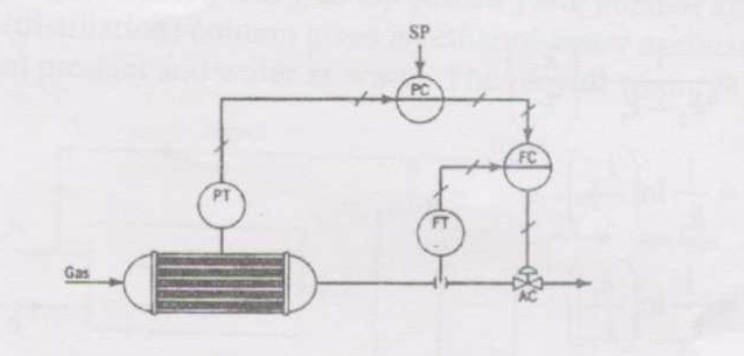
\includegraphics[width=0.5\columnwidth]{figs/71.png}
        \caption{}
        \label{fig:71}
    \end{figure}
The type of action for the two controllers are
\begin{enumerate}
    \item direct acting for the pressure control and direct acting for the flow control
    \item indirect acting for the pressure control and indirect acting for the flow control 
    \item direct acting for the pressure control and indirect acting for the flow control
    \item  indirect acting for the pressure control and direct acting for the flow control
\end{enumerate}

    \item The bias values for the two controllers, so that no offset occurs in either controller are

    \begin{enumerate}
        \item Pressure controller: 40\%; Flow controller: 60\%
        \item Pressure controller: 33\%; Flow controller: 67\%
        \item Pressure controller: 67\%; Flow controller: 33\%
        \item Pressure controller: 60\%; Flow controller: 40\%
    \end{enumerate}

    \item Given that the actual tank pressure is 4 bar(g) and a proportional controller is employed for pressure control, the proportional band setting of the pressure controller required to obtain a set point to the flow controller equal to$ 54 nm^3/hr$ is

\begin{multicols}{4}
    \begin{enumerate}
        \item 50\%
        \item 100\%
        \item 150\%
        \item 187\%
    \end{enumerate}
\end{multicols}

    \item The following liquid phase reaction is taking place in an isothermal batch reactor
    \begin{align*}
        A\xrightarrow{k_1\brak{first order}}B\xrightarrow{k_2\brak{zero order}}C
    \end{align*}
    Feed concentration = 1mol/litre
    The time at which the concentration of B will reach its maximum value is given by 

    \begin{enumerate}
        \item $t=\frac{1}{k_1}\ln{\frac{k_1}{k_2}}$
           \item $t=\frac{1}{k_2-k_1}\ln{\frac{k_2}{k_1}}$
              \item $t=\frac{1}{k_2}\ln{\frac{k_2}{k_1}}$
                 \item $t=\frac{1}{k_2}\ln{\frac{k_1}{k_2}}$
    \end{enumerate}

    \item The time at which the concentration of B will become zero is given by the following equation:

    \begin{multicols}{2}
        \begin{enumerate}
            \item $\brak{1-e^{-k_2t}}=k_2t$
            \item $t= \infty$
            \item $t=\frac{1}{k_2}$
            \item $t=\frac{1}{k_1}$
        \end{enumerate}
    \end{multicols}

    \item A methanol-water vapor liquid system is at equilibrium at $60\degree C$ and 60 kPa. The mole fraction of methanol in liquid is 0.5 and in vapor is 0.8. Vapor pressure of methanol and water at $60\degree C$ are 85 kPa and 20 kPa respectively. Assuming vapor phase to be an ideal gas mixture, what is the activity coefficient of water in the liquid phase?

\begin{multicols}{2}
    \begin{enumerate}
        \item 0.3
        \item 1.2
        \item 1.6
        \item 7.5
    \end{enumerate}
\end{multicols}

    \item What is the excess Gobbs free energy ($g^E$, in J/mol) of the liquid mixture?

    \begin{multicols}{2}
        \begin{enumerate}
            \item 9.7
            \item 388
            \item 422
            \item 3227
        \end{enumerate}
    \end{multicols}

    \item A simplified flowsheet is shown in the figure for production of ethanol from ethylene. The conversion of ethylene in the reactor is 30\% and the scrubber following the reactor completely separates ethylene (as top stream) and ethanol and water as bottoms. The last (distillation) column gives an ethanol-water azeotrope (90 mol\% ethanol) as the final product and water as waste. The recycle to purge ratio is 34.

\begin{figure}[H]
    \centering
    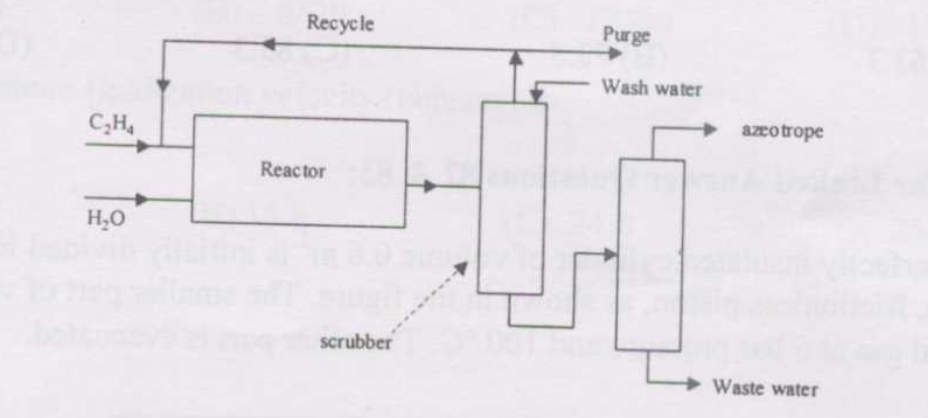
\includegraphics[width=0.5\columnwidth]{figs/78.png}
    \caption{}
    \label{fig:78}
\end{figure}

The reaction is: $C_2H_4\brak{g}+H_2O\brak{g}\to C_2H_5OH\brak{g}$

For an azeotrope product rate of 500 mols/hr, the recycle gas flowrate in mols/hr is 

\begin{multicols}{4}
    \begin{enumerate}
        \item 30
        \item 420
        \item 1020
        \item 1500
    \end{enumerate}
\end{multicols}

    \item For the same process, if fresh $H_2O$ feed to the reactor is 600 mol/hr and wash water for scrubbing is 20\% of the condensables coming out of the reactor, the water flowrate in mols/hr from the distillation column as bottoms is 

    \begin{multicols}{4}
        \begin{enumerate}
            \item 170
            \item 220
            \item 270
            \item 430
        \end{enumerate}
    \end{multicols}
\newpage
    \item 44kg of $C_3H_8$ is burnt with 1160 kg of air (Mol. Wt.=29) to produce 88kg of $CO_2$ and 14kg of $CO$
    \begin{align*}
        C_3H_8+5O_2=3CO_2+4H_2O
    \end{align*}
    What is the percent excess air used?

    \begin{multicols}{4}
        \begin{enumerate}
            \item 55
            \item 60
            \item 65
            \item 68
        \end{enumerate}
    \end{multicols}

    \item What is the \% carbon burnt?

    \begin{multicols}{4}
        \begin{enumerate}
            \item 63.3
            \item 73.3
            \item 83.3
            \item 93.3
        \end{enumerate}
    \end{multicols}

    \item A perfectly insulated cylinder of volume $0.6 m^3$ is initially divided into two parts by a thin, frictionless piston, as shown in the figure. The smaller part of volume $0.2 m^3$ has ideal gas at 6 bar pressure and $100\degree C$. The other part is evacuated.
    \begin{figure}[H]
        \centering
        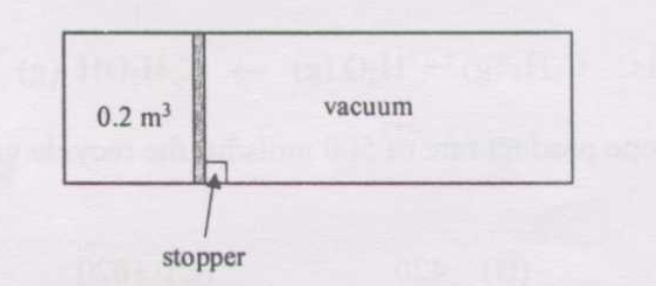
\includegraphics[width=0.5\columnwidth]{figs/82.png}
        \caption{}
        \label{fig:82}
    \end{figure}

At certain instant of time t, the stopper is removed and the piston moves out freely to

the other end. The final temperature is

\begin{multicols}{4}
    \begin{enumerate}
        \item $-149\degree C$
          \item $-33\degree C$
            \item $33\degree C$
              \item $100\degree C$
    \end{enumerate}
\end{multicols}

    \item The cylinder insulation is now removed and the piston is pushed back to restore the system to its initial state. If this is to be achieved only by doing work on the system (no heat addition, only heat removal allowed), what is the minimum work required?

    \begin{multicols}{4}
        \begin{enumerate}
            \item 3.4 kJ
            \item 107 kJ
            \item 132 kJ
            \item 240 kJ
        \end{enumerate}
    \end{multicols}

    \item A fluidized bed (0.5m dia, 0.5 high) of spherical particles ($diameter = 2000\mu m$, specific gravity = 2.5) uses water as the medium. The porosity of the bed is 0.4. The Ergun eqn for the system is 
    \begin{align*}
        \Delta P/L = 4\times 10^5 U_{mf}+1\times 10^7 U_{mf}^2 
    \end{align*}
    SI unit, $U_{mf}$ in m/s 
    
    $\Delta P/L$(SI unit) at minimum fluidization condition is 
    
    ($g=9.8m/sec^2$)

\begin{multicols}{4}
    \begin{enumerate}
        \item 900
        \item 8820
        \item 12400
        \item 17640
    \end{enumerate}
\end{multicols}

    \item The minimum fluidization velocity (mm/sec) is

 \begin{multicols}{4}
     \begin{enumerate}
         \item 12.8
         \item 15.8
         \item 24.8
         \item 28.8
     \end{enumerate}
 \end{multicols}














 \end{enumerate}

\end{document}